% ---------------------------------------------------------------------------- %

\section{Modelação de Domínio}
\label{cap:dominio}

Verificou-se que a construção do sistema seria vantajosa para a empresa e que o seu processo de desenvolvimento cumpriria o orçamento e prazos estabelecidos, reunindo-se assim as condições necessárias para se proceder à fase de especificação do mesmo.

Embora os procedimentos de modelação de domínio e de levantamento de requisitos sejam mutuamente dependentes, apresenta-se em primeiro lugar neste relatório o modelo de domínio por forma a clarificar a enunciação dos requisitos apresentados no próximo capítulo.

A abordagem utilizada para efetuar a modelação é baseada naquela apresentada por \textcite{sommerville2010software}, sendo utilizada a notação gráfica \emph{Unified Modeling Language} (UML)~\parencite{omg2017uml}, por representar a linguagem padrão para modelação orientada a objetos. 

A modelação de domínio foi efetuada em conjunto com o cliente do projeto, para garantir a correta estruturação do sistema, uma adequada nomenclatura que contribua para uma melhor perceção do sistema e que o sistema é apropriado para o seu objetivo.

\begin{figure}[ht]
  \centering
  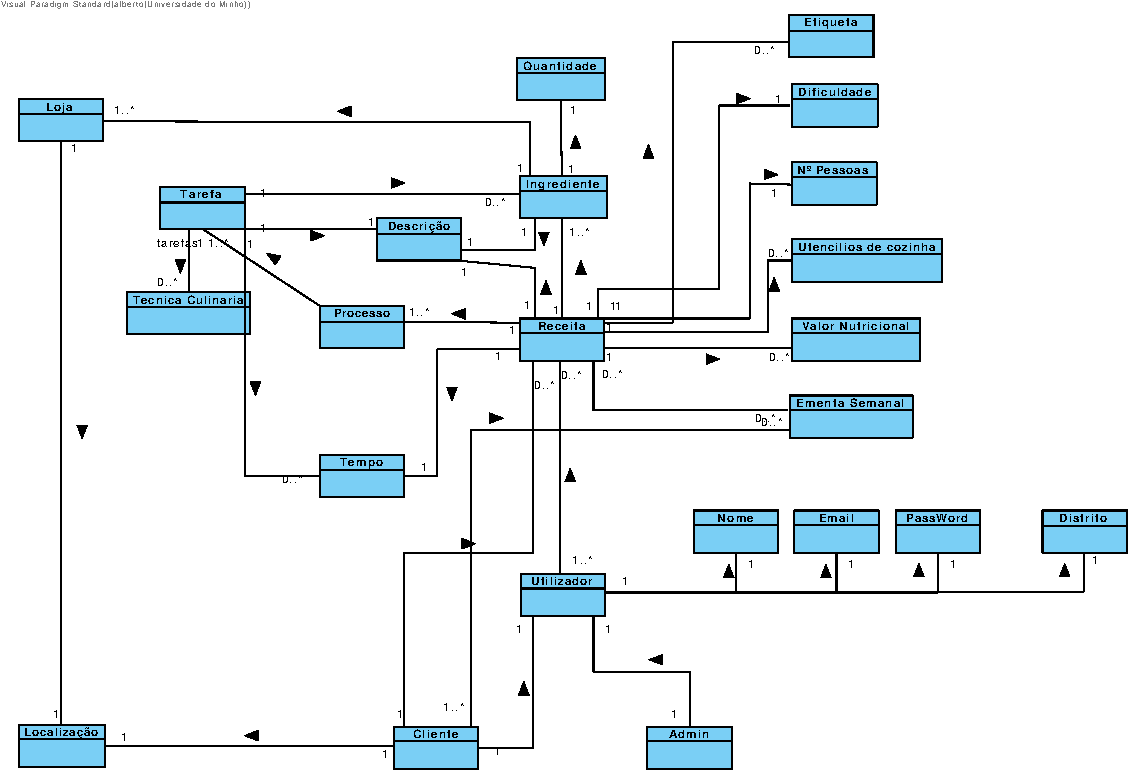
\includegraphics[width=\textwidth]{figures/04/diagrama-dominio.pdf}
  \caption{Diagrama do modelo de domínio.}
  \label{fig:dominio:diagrama}
\end{figure}

Decidiu-se que o sistema seria centrado na receita, que terá sempre uma proporção, uma dificuldade, vários ingredientes, técnicas e/ou utensílios de cozinha envolvidos, um conjunto de processos, cada um com um conjunto de tarefas que devem ser realizadas antes de prosseguir para o próximo processo, estando um tempo de execução e designação associada a cada tarefa e receita.
A receita também poderá ter valores nutricionais e etiquetas associadas a esta.

Quanto ao utilizador, este terá um nome, um email, uma palavra-passe e um distrito associado à sua conta pessoal, podendo este ser um cliente ou um administrador. Um cliente terá acesso a uma ementa semanal, com as receitas que pretende confecionar, para o almoço e jantar, nos dias de uma semana, e uma localização geográfica. 

A localização geográfica é também atribuída à loja onde o cliente poderá encontrar os diversos ingredientes usados nas receitas.

% ---------------------------------------------------------------------------- %

% Entidades:

%     - Utensílio
%     - Técnica
%     - Receita
%         - Tarefa
%             - Duração
%         - Dificuldade
%         - Quantidade de Porções
%         - Etiqueta
%         - Ingrediente
%         - Tempo de Preparação
%         - Valores Nutricionais
%     - Cliente
%         - Localização
%     - Administrador
%     - Utilizador
%         - Nome de Utilizador
%         - Palavra-Chave
%         - E-mail
%     - Histórico de Receitas Confecionadas
%     - Loja
%         - Localização
%     - Ementa Semanal

% Relacionamentos:

%     - Cliente é um Utilizador
%     - Administrador é um Utilizador

%     - Receita tem 1 Dificuldade
%     - Receita 1 tem 1..* Tarefa
%     - Receita serve 1 Quantidade de Porções
%     - Receita * é identificada por 1..* Etiqueta

%     - Cliente * tem interesse em * Etiqueta

%     - Cliente é identificado por 1 Nome de Utilizador

%     - Tarefa * faz uso de * Técnica

%     - Técnica * requer * Utensílio
%     - Passo * requer * Utensílio

% ---------------------------------------------------------------------------- %
